% arara: xelatex: { shell: yes }
% arara: biber
% arara: nomencl
% arara: xelatex: { shell: yes }
% arara: xelatex: { shell: yes }
\documentclass[ngerman]{ttlab-qualify}
% m�gliche Optionen:
% - ngerman
% - english
% - minted
% - algorithm
% - nomencl
% - nolibertine

%to export equation as png
%\usepackage[active,tightpage]{preview}
%\PreviewEnvironment{equation}

\usepackage{multirow}

\usepackage{ amssymb }
%\usepackage[captions=tableheadings]{booktabs}

\usepackage{listing} % pretty print code
\usepackage{lstbayes} % add stan languge support to listing

\usepackage{tikz}
\usepackage{subfigure}
\definecolor{light}{RGB}{220, 188, 188}
\definecolor{mid}{RGB}{185, 124, 124}
\definecolor{dark}{RGB}{143, 39, 39}
\definecolor{highlight}{RGB}{0, 255, 0}
\definecolor{gray10}{gray}{0.1}
\definecolor{gray20}{gray}{0.2}
\definecolor{gray30}{gray}{0.3}
\definecolor{gray40}{gray}{0.4}
\definecolor{gray60}{gray}{0.6}
\definecolor{gray70}{gray}{0.7}
\definecolor{gray80}{gray}{0.8}
\definecolor{gray90}{gray}{0.9}
\definecolor{gray95}{gray}{0.95}
\definecolor{comment}{gray}{0.50}

\addbibresource{bib/bayes.bib}
\usepackage{float} %use [H]with figure to place figures right in the text
 
\usepackage[colorlinks=false,
pdfpagelabels,
pdfstartview = FitH,
bookmarksopen = true,
bookmarksnumbered = true,
%urlcolor = blue,   %externe URLs
%linkcolor = black, %interne Verweise
%citecolor = blue,  %interne Zitate
urlbordercolor={0.5 0.5 0.5},
linkbordercolor={0.5 0.5 0.5},
citebordercolor={0.5 0.5 0.5},
plainpages = false,
hypertexnames = true]{hyperref}
%insert links from title back to toc
\makeatletter
\let\hyperchapter\chapter
\def\chapter{\@ifstar\starchapter\mychapter}
\def\starchapter{\hyperchapter*}
\newcommand{\mychapter}[2][\@empty]% #1=optional (toc and top of page), #2=title
{\ifx#1\@empty \hyperchapter[#2]{\hyperlink{toc.chapter.\thechapter}{#2}}
 \else \hyperchapter[#1]{\hyperlink{toc.chapter.\thechapter}{#2}}
 \fi}

\let\hypersection\section
\def\section{\@ifstar\starsection\mysection}
\def\starsection{\hypersection*}
\newcommand{\mysection}[2][\@empty]% #1=optional (toc), #2=title
{\ifx#1\@empty \hypersection[#2]{\hyperlink{toc.section.\thesection}{#2}}
 \else \hypersecton[#1]{\hyperlink{toc.section.\thesection}{#2}}
 \fi}
 
 \let\hypersubsection\subsection
\def\subsection{\@ifstar\starsubsection\mysubsection}
\def\starsubsection{\hypersubsection*}
\newcommand{\mysubsection}[2][\@empty]% #1=optional (toc), #2=title
{\ifx#1\@empty \hypersubsection[#2]{\hyperlink{toc.subsection.\thesubsection}{#2}}
 \else \hypersubsecton[#1]{\hyperlink{toc.subsection.\thesubsection}{#2}}
 \fi}
\makeatother
%change u.a. to et.al. - edit E. Fughe 4.7.18
\DefineBibliographyStrings{ngerman}{
   andothers = {{et\,al\adddot}},
}

\begin{document}
\let\hypercontentsline=\contentsline
\renewcommand{\contentsline}[4]{\hypertarget{toc.#4}{}\hypercontentsline{#1}{#2}{#3}{#4}}

\titlehead{
  Elisabeth Fughe\\
  Matrikelnummer: 5263769\\
  s3499227@stud.uni-frankfurt.de
}
\subject{Bachelorarbeit (B.Sc. - Informatik)}
\author{Elisabeth Fughe}
\title{Können Modelle der Ökonophysik Preis-Dynamiken vorhersagen?}
\subtitle{Fitting von Markt-Modellen auf empirischen Daten mittels Bayesscher Statistik}
\date{Abgabedatum: 16. April 2019}
\publishers{FIAS - Frankfurt Institute for Advanced Studies\\Prof. Dr. Nils Bertschinger}
%\\Ggf. Name des Zweitbetreuers}

\maketitle

\chapter*{Zusammenfassung}
tbd

\tableofcontents
%\listoffigures
%\listoftables

\chapter{Einleitung}
\label{chap:summary}
tbd

\chapter{Verwendete Methoden}
\label{chap:methoden}
tbd
\section{Bayessche Modellierung}
Die Bayessche Statistik untersucht mittels Bayesscher Wahrscheinlichkeiten und dem Satz von Bayes Fragestellungen der Stochastik. Anders als in der klassischen Statistik, die unendlich oft wiederholbare Zufallsexperimente voraussetzt, steht die Verwendung und Modellierung von Wahrscheinlichkeitsverteilungen im Vordergrund. \\
Es gilt, das beobachtete Daten 
\[x=(x_1,...,x_n)\] 
mittels bedingter Wahrscheinlichkeiten in Beziehung zu unbekannten Parametern 
\[\theta = (\theta_1,...,\theta_m)\] 
stehen. So kann die gemeinsame Wahrscheinlichkeitsdichte 
\[p(x,\theta) = p(x|\theta)\cdot p(\theta)\]
durch die a-priori-Verteilung unbekannter Parameter $p(\theta)$ und den Erkenntnissen aus dem Datensatz $p(x|\theta)$ berechnet werden.
Mit Hilfes des Satzes von Bayes kann dann die a-posteriori-Verteilung unbekannter Parameter 
\[p(\theta|x) =\dfrac{p(x|\theta)\cdot p(\theta)}{p(x)}\] 
ermittelt werden \parencite{bertschinger:2018}.

Die a-posteriori-Verteilung enthält somit Informationen über die unbekannten Parameter durch die Kombination der a-priori Verteilung mit den Informationen, die aus den beobachteten Daten gewonnen wurden. Sie wird zur Punktschätzung und Schätzung von Konfidenzintervallen genutzt und daher auch oft als Ziel-Verteilung bezeichnet.

So sind Bayessche Modelle im Gegensatz zur klassischen Statistik auf kleineren Datensätzen anwendbar, dort ergibt sich jedoch eine breite Wahrscheinlichkeitsverteilung, die somit unter Umständen eine geringe Genauigkeit aufweist.

\section{Markov Chain Monte Carlo (MCMC)}
\label{chap:MCMC}
In der Bayesschen Statistik beschreibt die a-posteriori-Verteilung die Unsicherheit der unbekannten Parameter, die anhand beobachteter Daten geschätzt wurden. Mit der Markov Chain Monte Carlo (MCMC) Methode kann die a-posteriori-Verteilung und somit die unbekannten Parameter  untersucht werden \parencite{hanson:2001}.

Um aus der Ziel-Verteilung Stichproben ziehen zu können wird eine Markov-Kette entworfen, deren stationäre Verteilung der Ziel-Verteilung entspricht. Hier wird eine Stichprobe aus der a-posteriori-Wahrscheinlichkeitsdichte benötigt, sodass das langfristige Gleichgewicht der Markov-Kette der a-posteriori-Wahrscheinlichkeitsdichte entspricht. Der Zustand der Markov-Kette, der sich möglichst nah am Gleichgewicht befindet, entspricht dann einem Element der Stichprobe. Es gilt somit, dass sich die Qualität der Stichprobe mit der Anzahl der Schritte, die die Markov-Kette zurücklegt, verbessert.\\

Zur Konstruktion der Markov-Kette wird eine Übergangsfunktion berechnet, die die Ziel-Wahrscheinlichkeitsdichte invariant lässt, damit die Ziel-Dichte der stationären Verteilung der Markov-Kette entspricht. 
Sei z.B. $p(\theta)$ die Ziel-Dichte und sei $t(\theta^{'}|\theta)$ die Übergangsdichte, dann gilt
\[p(\theta^{'}) =\int t(\theta^{'}|\theta)\cdot p(\theta) d\theta \]

Stellt man sich die Markov-Kette als zufällig durch einen Parameterraum, also z.B. die a-posteriori-Verteilung, wandernden Punkt vor, so entspricht die $n$-te Komponente der Verteilung der relative Wahrscheinlichkeit, den Punkt im Zustand $n$ anzutreffen. 
%insert figure from betancourt:2017
\begin{figure}[h]
\begin{center}
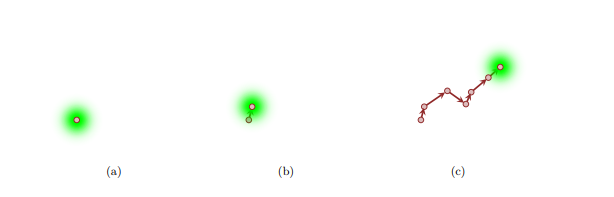
\includegraphics[scale=.9]{images/markov-chain-plain-betancourt-2017}
\caption{Verhalten der Markov-Kette beim Ziehen von Stichproben \parencite{betancourt:2017}}
\label{fig:markov-chain-plain}
\end{center}
\end{figure}

Die Übergangsdichte (grün) (a) in Abbildung~\ref{fig:markov-chain-plain} beschreibt die Wahrscheinlichkeit eines neuen Punktes im Parameterraum in Abhängigkeit der aktuellen Position. D.h. die Wahrscheinlichkeit des nächsten Schrittes der Markov-Kette auf ihrem Weg durch die Verteilung in Abhängigkeit ihrer aktuellen Position.  Werden Stichproben aus dieser Verteilung gezogen, also wurden zufällig gewählte nächste Schritte vom Algorithmus akzeptiert, ergibt sich ein weiterer Zustand in der Markov-Kette und eine neue Verteilung von der Stichproben gezogen werden können (vgl. (b) in Abbildung~\ref{fig:markov-chain-plain}). So wandert die Markov-Kette durch den Parameterraum (c) in Abbildung~\ref{fig:markov-chain-plain}.

\begin{figure}[H]
\begin{center}
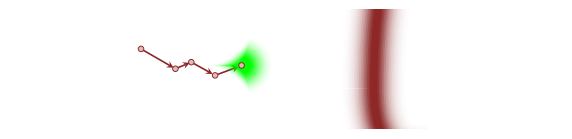
\includegraphics[scale=.9]{images/markov-chain-target-betancourt-2017}
\caption{Konzentration der Markov-Kette auf die typische Menge einer Verteilung \parencite{betancourt:2017}}
\label{fig:markov-chain-target}
\end{center}
\end{figure}

Wenn die Übergangsdichte die Ziel-Verteilung beibehalten soll, konzentriert sie sich auf deren typische Menge\footnote{\textbf{Typical Set (hier: typische Menge):} Die typische Menge ist ein Begriff aus der Informationstheorie und hängt direkt mit dem Begriff der Entropie zusammen. Es gilt, dass die Summe aller Wahrscheinlichkeiten aller Elemente der typischen Menge annähernd 1 ist \parencite{typical_set}. Daher enthält die typische Menge eine gute Beschreibung des Parameterraums.} (rot) siehe Abbildung~\ref{fig:markov-chain-target}. 
Unter idealen Bedingungen entdeckt die Markov-Kette in drei verschiedenen Phasen:
\begin{enumerate}
\item Die Markov-Kette konvergiert gegen die typische Menge der Verteilung. Die MCMC-Schätzer sind stark verzerrt.
\item Die Markov-Kette hat die typische Menge erkannt und verweilt dort. Diese erste Erkundung der typischen Menge ist äußerst effektiv und verringert die Verzerrung der MCMC-Schätzer erheblich, da die Verzerrung der ersten Stichproben eliminiert wird.
\item In der dritten Phase wird die Präzision der MCMC-Schätzer durch weiteres Erforschen der typischen Menge weiter verfeinert, so dass sie den zentralen Grenzwertsatz erfüllen. Das bedeutet, dass die durch die Markov-Kette gezogenen Stichproben asymptotisch der Ziel-Verteilung folgen.
\end{enumerate}

Ideale Bedingungen liegen allerdings nicht vor, wenn die typische Menge der a-posteriori-Verteilung z.B. eine starke Krümmung aufweist (siehe Abbildung~\ref{fig:markov-chain-curve}). Die Markov-Kette kann damit nicht umgehen und aus diesem stark gekrümmten Bereich keine Stichprobe ziehen und ignoriert diesen einfach und verzerrt dadurch die MCMC-Schätzer. 
Da Markov-Ketten die exakten Erwartungen asymptotisch wiederherstellen müssen, ist eine Kompensation dafür nötig, dass manche Regionen der Ziel-Verteilung nicht beachtet wurden. Dazu bleibt die Markov-Kette an der Grenze der Krümmung hängen. So werden die MCMC-Schätzer annähernd so berechnet, als würde die Markov-Kette den gekrümmten Bereich erkunden. Allerdings erhält man so überschätzte MCMC-Schätzer.
Eine starke Krümmung in der typischen Menge der Ziel-Verteilung führt also zu verzerrten MCMC-Schätzern, die den zentralen Grenzwertsatz nicht mehr erfüllen \parencite{betancourt:2017}.

\begin{figure}[H]
\begin{center}

\includegraphics[scale=.9]{images/markov-chain-curve-betancourt-2017}
\caption{Starke Krümmungen (grün) der typischen Menge einer Verteilung führen zu verzerrten MCMC-Schätzern \parencite{betancourt:2017}}
\label{fig:markov-chain-curve}
\end{center}
\end{figure}


%----

%Anschließend wird diese Markov-Kette solang simuliert bis sie, mit einer entsprechenden Sicherheit, das Gleichgewicht erreicht hat. Dann wird der finale Zustand der Markov-Kette als Teil der Stichprobe notiert \parencite{kendall:2005}. Die Markov-Kette generiert so eine Reihe von Modell-Realisierungen, die zufällig aus der a-posteriori-Verteilung gezogen werden \parencite{hanson:2001}.\\

Ein weit verbreitetes MCMC-Verfahren zur Konzentration auf die typische Menge der zu untersuchenden Verteilung ist der Metropolis-Hastings-Algorithmus. Der Algorithmus startet an einem zufälligen Punkt in der zu untersuchenden Verteilung.
Dann wird eine Schrittweite zufällig mit Hilfe einer symmetrischen Wahrscheinlichkeitsverteilung gewählt.
Der Schritt wird auf Grundlage der Wahrscheinlichkeit der neuen Position im Verhältnis zur alten Position abgelehnt oder akzeptiert \parencite{hanson:2001}.
So wird sicher gestellt, dass die Markov-Kette von jedem Punkt aus gegen das langfristige Gleichgewicht der Ziel-Wahrscheinlichkeitsdichte konvergiert \parencite{bertschinger:2018}.\\

Der Metropolis-Hastings-Algorithmus ist sehr einfach zu implementieren und liefert gute Ergebnisse, allerdings nicht bei stark korrelierten Parametern \parencite{hanson:2001} und hoher Komplexität der Verteilung \parencite{betancourt:2017}.  Denn wenn die a-posteriori-Verteilung stark gekrümmt ist, bleibt die Markov-Kette an diesen Rändern hängen und lehnt so gut wie jeden weiteren Schritt ab. So kann nicht aus allen Bereiche der Ziel-Verteilung Stichproben gezogen werden und es entsteht eine verzerrte Stichprobe.\\
Je mehr Dimensionen die Verteilung hat, desto kleiner wird die typische Menge der Verteilung. Das führt dazu, dass fast immer Punkte außerhalb der typischen Menge gewählt werden. Die Dichte des Punkts ist so klein, dass der Schritt vom Metropolis-Hastings-Algorithmus immer abgelehnt wird. Das führt dazu, dass sich die Markov-Kette kaum weiter bewegt. Erhöht man die Akzeptanz, indem man die Anzahl der Punkte reduziert, die sich in der typischen Menge befinden müssen, aber das führt dazu, dass die Markov-Kette extrem langsam konvergiert \parencite{betancourt:2017}. In der Theorie würde die Markov-Kette das langfristige Gleichgewicht erreichen, aber in der Praxis stehen dazu nicht unendliche Ressourcen zur Berechnung zur Verfügung. \\
%not sure
Der Metropolis-Hastings-Algorithmus kann auch als stochastisches Optimierungsverfahren verstanden werden. Mittels Simulated Annealing\footnote{\textbf{Simulated Annealing:} \glqq Ein heuristisches Approximationsverfahren. Es wird zum Auffinden einer Näherungslösung von Optimierungsproblemen eingesetzt, die durch ihre hohe Komplexität das vollständige Ausprobieren aller Möglichkeiten und mathematische Optimierungsverfahren ausschließen\grqq \parencite{simulated_annealing}.} nähert man sich mit immer höherer Wahrscheinlichkeit an ein Minimum an. Ist die Krümmung der Verteilung zu stark, kann der Algorithmus das lokale Minimum nicht mehr verlassen und so wird fast jeder weitere Schritt der Markov-Kette immer abgelehnt. Letztlich wird der Bereich der Verteilung ignoriert bzw. die Markov-Kette bleibt am Rand des unerwarteten Bereichs hängen. Das führt zu einer Verzerrung der resultierenden MCMC-Schätzer \parencite{betancourt:2017}.

\section{Hamiltonian Monte Carlo Sampling (HMC)}
\label{chap:HMC}
In Modellen mit vielen Dimensionen ist es möglich, dass die Markov-Kette mittels Metropolis-Hastings-Algorithmus nicht alle Bereiche der Ziel-Verteilung in einer angemessenen Zeit abtasten kann. 
Die Strategie des Metropolis-Algorithmus, zufällige Schritte zu wählen und danach zu entscheiden, ob der Schritt akzeptiert wird oder nicht, ist für Modelle mit vielen Dimensionen weniger erfolgreich. Denn es existieren exponentiell viele Richtungen, in die sich der Sampler bewegen kann, aber nur ein Bruchteil der Richtungen belässt den Sampler in der typischen Menge und führt letztlich zu akzeptieren Stichproben.\\

Um also große Schritte vom initialen Punkt in unentdeckte Bereiche der Ziel-Verteilung machen zu können, müssen Informationen über die Geometrie der Verteilung genutzt werden. Die Markov-Kette soll Übergänge berechnen, die der Masse mit hohen Wahrscheinlichkeiten folgt, sich also zusammenhängend durch die typische Menge bewegen. Diese Hamiltonian-Markov-Übergänge können durch Nutzung der differenzierbaren Struktur der a-posteriori-Verteilung berechnet werden.\\

\begin{figure}[H]
\begin{center}
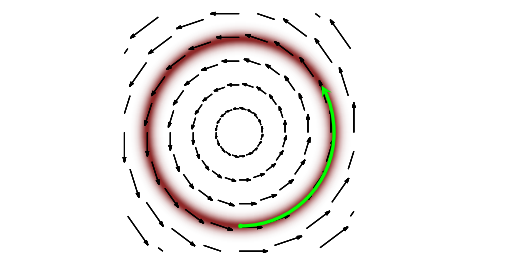
\includegraphics[scale=.9]{images/vector-field-plain-betancourt-2017}
\caption{Mit Hilfe eines Vektorfeldes das an der typischen Menge ausgerichtet ist, kann die Ziel-Verteilung leichter abgetastet werden \parencite{betancourt:2017}.}
\label{fig:vec-field-plain}
\end{center}
\end{figure}

Um die Zielverteilung schneller und gezielter abtasten zu können, wird jedem Punkt im Parameterraum eine Richtung für eine kleine Distanz zugewiesen, z.B. durch ein Vektorfeld, dass an der typischen Menge ausgerichtet ist (vgl. Abbildung~\ref{fig:vec-field-plain}). Folgt der Sampler den Richtungen, entsteht eine zusammenhängende Kurve (\textit{engl. Trajectory}), die effizient und möglichst schnell vom initialen Punkt durch unentdeckte Bereiche  der typischer Menge der Ziel-Verteilung führt \parencite{betancourt:2017}.\\

Um jedem Punkt eine Richtung zuzuweisen, kann ein Vektorraum mittels Informationen der Ziel-Verteilung konstruiert werden. Dazu wird die differenzielle geometrische Struktur der a-posteriori-Verteilung benötigt, die wir durch den Gradienten der Ziel-Dichte erhalten können. Denn der Gradient der Ziel-Dichte definiert eben ein solches für die geometrische Struktur der Verteilung sensitives Vektorfeld im Parameterraum.

\begin{figure}[H]
\begin{center}
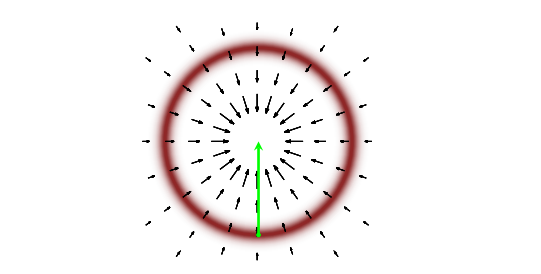
\includegraphics[scale=.9]{images/vector-field-grad-betancourt-2017}
\caption{Die Richtung des Gradienten zeigt immer von der typischen Menge in Richtung parameter-sensitiver Bereiche(grüner Pfeil), wie z.B. dem Modus der Verteilung. Folgt der Sampler diesen Richtungen, kann er die typische Menge nicht erkunden \parencite{betancourt:2017}.}
\label{fig:vec-field-grad}
\end{center}
\end{figure}

Allerdings hängen Ziel-Dichte sowie ihr Gradient stark von den Verteilungsparametern ab, sodass der Gradient immer in Richtung parameter-sensitiver Bereiche wie z.B. dem Modus\footnote{\textbf{Modus:} Der Modus ist ein Begriff der desktiptiven Statistik. Er entspricht dem häufigsten Wert einer Stichprobe \parencite{modus}.} der Verteilung zeigt (vgl. Abbildung~\ref{fig:vec-field-grad}).
Das Vektorfeld enthält somit nicht genügend Informationen, um den Sampler durch die typische Menge in parameter-invariante Bereiche zu führen. Um parameter-invariante Bereiche der Ziel-Dichte zu erkunden, muss der Gradient um zusätzliche geometrische Informationen ergänzt werden. \\

Das Ergänzen der Informationen ist durch Differentialgeometrie möglich, die auch die Mathematik der klassischen Physik beschreibt. Es gilt, dass für jedes probabilistische System ein mathematisch äquivalentes physikalisches System existiert \parencite{betancourt:2017}.
Das Erkunden der Ziel-Dichte kann äquivalent auch als Erkunden eines physikalischen Systems beschrieben werden. Sei der Modus der Ziel-Dichte ein Planet und der Gradient sein Gravitationsfeld, dann sei die typische Menge der Dichte, der Bereich um den Planet, durch den ein Satellit kreisen soll (vgl. Abbildung~\ref{fig:vec-field-sat}). \\

\begin{figure}[H]
\begin{center}
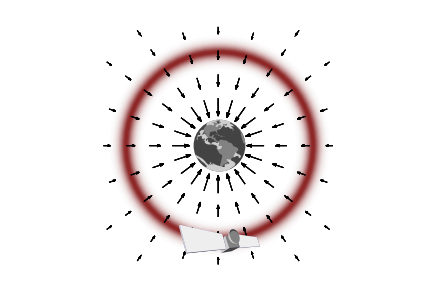
\includegraphics[scale=.9]{images/vector-field-sat-betancourt-2017}
\caption{Analoges System der klassischen Physik \parencite{betancourt:2017}.}
\label{fig:vec-field-sat}
\end{center}
\end{figure}

Es gilt also das probabilistische Modell so um Impulse (\textit{engl. Momentum}) zu erweitern, dass analog der Satellit die Anziehungskraft des Planeten ausbalanciert und die gewünschte Umlaufbahn nicht verlässt \parencite{betancourt:2017}. Der Hamiltonian Monte Carlo Algorithmus ist der einzige Algorithmus, der Impulse mit einer probabilistischen Struktur, die konservative Dynamiken erlaubt, implementiert \parencite{betancourt:2017}.\\

Der HMC-Algorithmus zieht also Stichproben aus einem erweiterten Zustandsraum mit Impuls $i$ eines Teilchens an der Position $P$.\\
Für die Dichte $d(P,i)$ des Zustandsraums gilt \parencite{bertschinger:2018}:
\begin{align}
d(P,i)&= d(P)d(i|P)\nonumber\\
&=e^{log\; d(P)+log\; d(i|P)}\nonumber\\
&=e^{-H(P,i)}
\end{align}
Wobei die Hamiltonian-Korrektur $H(P,i)$ in Analogie zum physikalischen System der Summe potentieller und kinetischer Energie entspricht.
\[H(P,i) = -log\; d(P)-log\; d(i|P)\]
Die Hamiltonian Dynamiken $\hat{P}$ und $\hat{i}$
\begin{align} \label{eq:hamiltonian-dynamics}
\hat{P}&= \frac{\partial}{\partial i}H(P,i) \nonumber\\
&= -\frac{\partial}{\partial i} log\; d(i|P) \nonumber \\
&\nonumber\\
\hat{i}&=-\frac{\partial}{\partial P}H(P,i)\nonumber\\
&=\frac{\partial}{\partial P}log\; d(P) + \frac{\partial}{\partial P}log\; d(i|P)
\end{align}
erhalten die gesamte Energie bzw. Wahrscheinlichkeit und so kann beim HMC Sampling stets ein Schritt berechnet werden, der akzeptiert wird \parencite{bertschinger:2018}, sodass die Markov-Kette auch aus stark gekrümmten Bereichen akzeptierte Stichproben ziehen kann. Besonders in Modellen mit vielen Dimensionen schafft das HMC Sampling so wichtige Effizienzvorteile.\\

Theoretisch ist HMC Sampling unempfindlich bezüglich stark korrelierter Parameter, allerdings werden die Differenzialgleichungen in der Praxis mittels endlicher Schrittweite gelöst. Das kann dazu führen, dass stark gekrümmte Bereiche der Ziel-Dichte doch nicht mehr erreicht werden. Außerdem gilt es die Schrittweite entsprechend der Parameter-Maßeinheiten und -größen anzupassen \parencite{bertschinger:2018}. 

\section{\textit{Stan} und \textit{R}}
\label{chap:stan}
\textit{Stan} ist eine Open-Source Plattform für statistische Modellierung und high-performance Berechnungen. 
\textit{Stan} ist für alle in der Datenanalyse weit verbreiteten Sprachen (R, Python, shell MATLAB, Julia, Stata) verfügbar und läuft auf den gängigen Betriebssystem (Linux, Mac, Windows) \parencite{stan:2017}. \\

\textit{Stan} ist eine höhere Programmiersprache und ermöglicht die Beschreibung der gemeinsamen Verteilung eines Modells auf einer hohen Abstraktionsebene. Die Sprache unterstützt viele Inferenz-Algorithmen, insbesondere Algorithmen die das Gradientenabstiegsverfahren nutzen, um eine maximale a-posteriori-Schätzung zu erhalten, HMC Sampling sowie Bayessche Gradientenvariation (stochastic gradient variational Bayes). \textit{Stan} Code wird in C++ kompiliert und die hohe Abstraktionsebene der Sprache bietet dem Nutzer einige Vorteile, z.B. müssen bei der Nutzung von HMC Sampling die Gradienten nicht manuell implementiert werden. Benötigte Gradienten werden built-in mittels C++ Library für automatisches Differenzieren berechnet werden \parencite{bertschinger:2018}.\\

Ein \textit{Stan}-Programm muss mindestens einen \verb|data|-, einen \verb|Parameter|-Block sowie einen \verb|model|-Block enthalten.
Ein Beispiel dafür ist der \textit{Stan}-Code des in dieser Arbeit verwendeten GARCH-Modells:\\

Im \verb|data|-Block wird definiert, welche Daten benötigt werden, um das Modell zu fitten. Die Variablen in diesem Block entsprechen also den tatsächlichen Beobachtungen und der Block definiert, in welchem Format diese Daten vorliegen.\\
Hier werden zum Beispiel ein Vektor mit Zeitpunkten \verb|T|, ein Vektor mit Angabe, ob es sich um eine tatsächliche Beobachtung oder um einen zu vorhersagenden Wert handelt, sowie einen Vektor der beobachteten Returns in jedem Zeitpunkt.\\

Im \verb|transformed data| Block können berechnete Daten/Variablen definiert werden. Hier zum Beispiel wird über die Daten iteriert und festgestellt, wie viele Einträge als \textit{Missing Value} markiert wurden. So werden Beobachtungen und zu vorhersagende Daten unterschieden.

\begin{lstlisting}[language=Stan]
data {
  int<lower=0> T;
  int<lower=0, upper=1> miss_mask[T];
  real ret_obs[T]; // Note: Masked indices treated as missing
}
transformed data {
  int N = 0; // number of missing values
  for (t in 1:T)
    if (miss_mask[t] == 1) N = N + 1;
}

\end{lstlisting}

Daran anschließend kommt der \verb|parameters|-Block, der die unbekannten Parameter des Modells definiert. Anschließend daran kann der \verb|transformed parameters|-Block dazu genutzt werden, um z.B. die Berechnungsvorschrift weiterer Parameter festzulegen.\\

Hier wird der Return für jeden Zeitpunkt \verb|T| berechnet: Handelt es sich um eine tatsächliche Beobachtung, wird der beobachtete Return genommen, ansonsten erfolgt dier Berechnung mit Hilfe der Standardabweichung im aktuellen Zeitpunkt berechnet:\\
\verb|ret[t] = mu + sigma[t] * eps_miss[t]|

\begin{lstlisting}[language=Stan]
parameters {
  real mu;
  real<lower=0> alpha0;
  real<lower=0,upper=1> alpha1;
  real<lower=0,upper=(1-alpha1)> beta1;
  real<lower=0> sigma1;
  real eps_miss[N]; // missing normalized return innovations
}
transformed parameters {
  real ret[T]; // returns ... observed or r_t = mu + sigma_t * eps_t
  real<lower=0> sigma[T];

  {
    int idx = 1; // missing value index

    sigma[1] = sigma1;
    if (miss_mask[1] == 1) {
      ret[1] = mu + sigma[1] * eps_miss[idx];
      idx = idx + 1;
    } else
      ret[1] = ret_obs[1];

    for (t in 2:T) {
      sigma[t] = sqrt(alpha0
                    + alpha1 * pow(ret[t - 1] - mu, 2)
                    + beta1 * pow(sigma[t - 1], 2));
      if (miss_mask[t] == 1) {
        ret[t] = mu + sigma[t] * eps_miss[idx];
        idx = idx + 1;
      } else
        ret[t] = ret_obs[t];
    }
  }
}
\end{lstlisting}

Zum Schluss kommt der \verb|model|-Block, der die Berechnungsvorschrift der Wahrscheinlichkeitsdichte des Modells enthält \parencite{stan:2017}.\\
Hier die Annahme, dass \verb|mu| und \verb|sigma| standardnormalverteilt sind. Die Returns sind normalverteilt zu den Parametern des Modells (\verb|mu|, \verb|sigma|) wobei es sich, um die Standarabweichung in jedem Zeitpunkt \verb|T| handelt. Weitere Erläuterungen befinden sich im Kapitel~\ref{chap:garch} \\

Anschließend daran können im \verb|generated quantities|-Block weitere Berechnungen definiert werden. 
Hier z.B. die Berechnungsvorschrift der bedingten gemeinsamen Wahrscheinlichkeitsdichte.

\begin{lstlisting}[language=Stan]
model {
  mu ~ normal(0, 1);
  sigma1 ~ normal(0, 1);

  ret ~ normal(mu, sigma);
  // Jacobian correction for transformed innovations
  for (t in 1:T) {
    if (miss_mask[t] == 1)
      target += log(sigma[t]);
  }
}
generated quantities {
  real log_lik[T];

  for (t in 1:T)
    log_lik[t] = normal_lpdf(ret_obs[t] | mu, sigma[t]);
}

\end{lstlisting}

Der \textit{Stan}-Code der Modelle, die in dieser Arbeit genutzt wurden befindet sich im Anhang und wird im Kapitel~\ref{chap:models} näher erläutert.


Die Modelle wurden mittels \textit{Rstan} in \textit{R} gefittet. \textit{Rstan} ermöglicht es \textit{Stan}-Modelle in \textit{R} zu kompilieren, zu testen und zu analysieren. 
Außerdem wurden die Pakete \textit{tidybayes} und \textit{tidyverse} genutzt, um die Plots zu generieren. Die tidy* Pakete zeichnen sich dadurch aus, dass sie der komplexen Datenstruktur des berechneten Fits, Informationen leicht entnehmen können und in einer Datenstruktur zur Verfügung stellen, die anschließend z.B. mittels \textit{ggplot}-Packet leicht in \textit{R} visualisiert werden kann.

\chapter{Die Modelle}
\label{chap:models}
tbd
\section{GARCH}
\label{chap:garch}
tbd

\section{Vikram \& Sinha (VS)}
tbd maybe

\section{Franke \& Westerhoff (FW)}
\label{chap:FW}
tbd\\

random walk - treedepth 128 ?!

\section{AL herd walk (AL)}
\label{chap:AL}
tbd

\chapter{Simulationen}
\label{chap:sim}
tbd

\section{Daten \& Vorhersagen}
\label{chap:data}
S\&P 500 data in USD from finance.yahhoo: \\ 
-daily prices - calculated into return and finally into log return as models expect log return as inputs\\
-exporting data with dates like Jan 1 2000 to Jan 1 2008 yahoo automatically uses last working day at stock exchange\\
- always used 30 Predictions - inaccurate as days per month change\\
=> this all leads to inaccurancy which is ok as the goal is to see the tendency in which way predictions are shifting \\\\
monthly prediction during a year in which a major crisis happend: bank crisis 2008 \& dotcom 2000?\\
used 8 years to predict the year 2008 on a monthly basis: e.g. data from Jan 1 2000 to Jan 1 2008 used to predict Jan 2008

\section{Ergebnisse}
\label{chap:results}
tbd

\includegraphics[scale=.6]{../plots/bank-crisis/AL_walk/01_AL_walk_Jan_low_info_depth-13_delta_9}

\appendix
\printbibliography
\listoffigures
\end{document}

